\chapter{Theoretical Background and Related Work}
\label{lit_rec}

This chapter reviews the domain of historical document analysis and the role of text line segmentation within it,
expands on the theses mentioned in Section \ref{sec:motivation}, describes Few-shot learning essentials, explains how it intersects with text line segmentation in historical documents, and formulates the research gap.

\section{Historical Document Analysis}

Historical document analysis is a research field focused on digitizing, processing, and extracting information from historical documents, whether for content extraction or metadata analysis, such as authorship identification.

\begin{figure}[H]
    \centering
    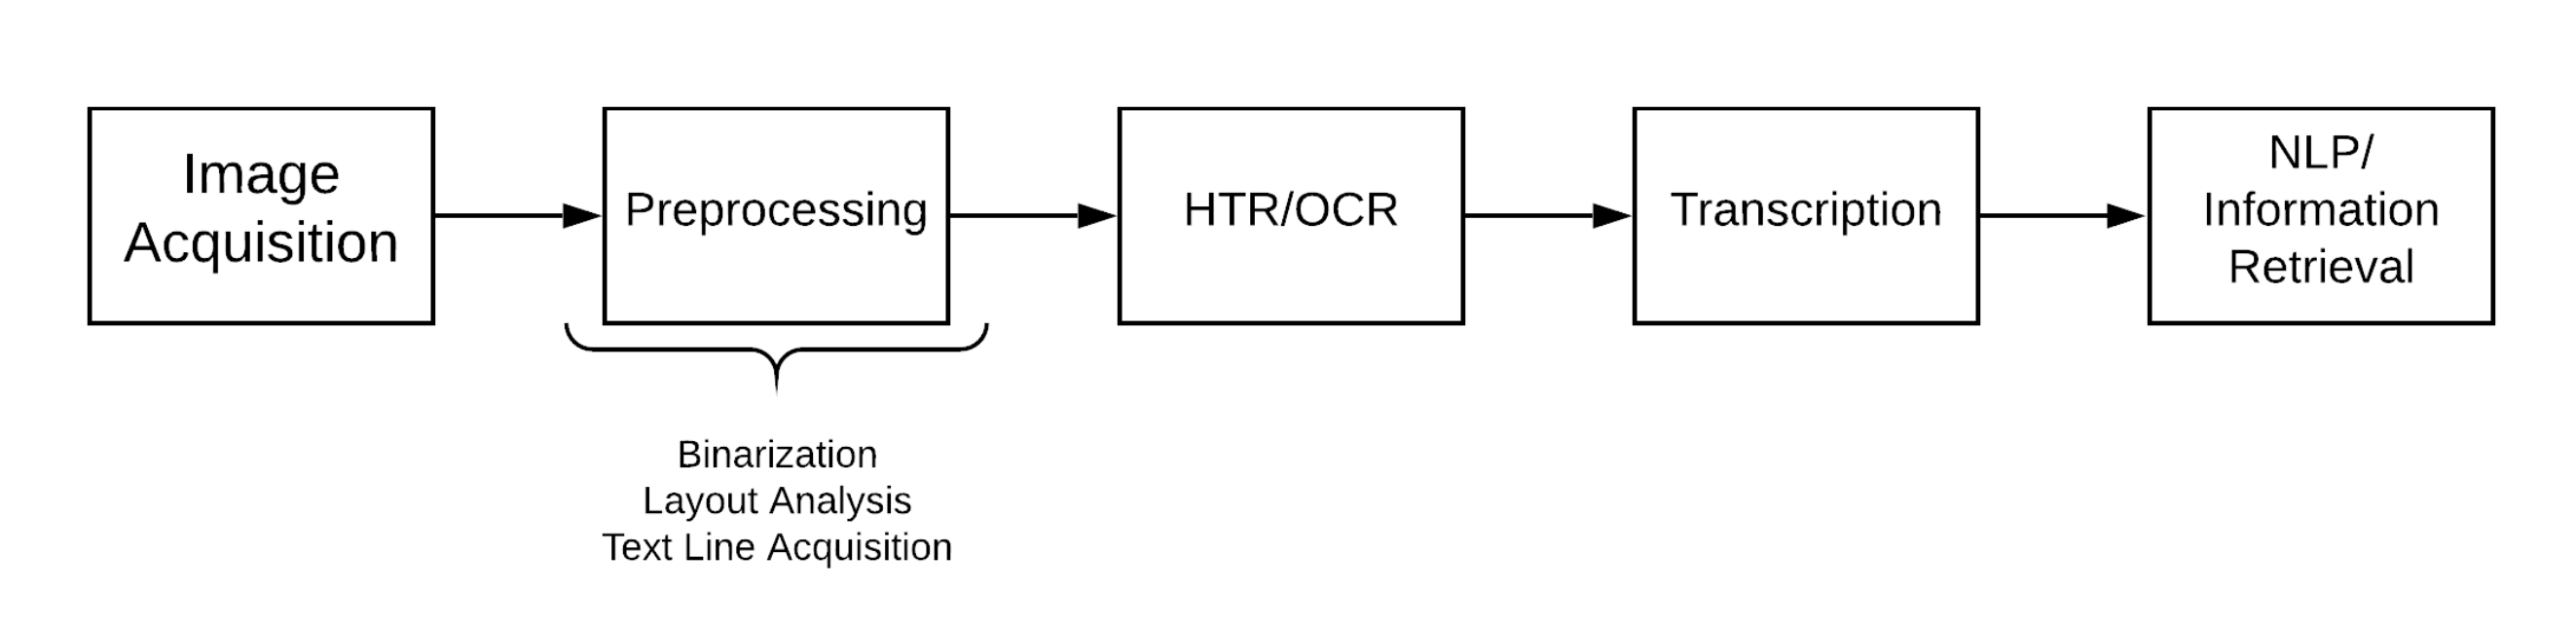
\includegraphics[width=1\linewidth]{graphics/Screenshot from 2026-06-21 13-06-12.png}
    \caption{The steps in a conventional Historical Document Processing workflow for both handwritten and printed documents, reproduced from \cite{DBLP:journals/corr/abs-2002-06300}}
    \label{fig:da_steps}
\end{figure}

Historical document analysis typically involves multiple stages, as shown in Figure \ref{fig:da_steps}. In the pipeline, historical materials pose several challenges because their visual appearance and layout can differ markedly between collections. Frequent issues include uneven line spacing, different text orientations, notes in the margins, stains, bleed-through, and characters or text lines that touch or overlap \cite{Rabaev_Litvak_2025}. Figure \ref{fig:hda_challenges} shows general layout- and degradation-related problems, along with examples of overlapping and deteriorated text line regions.
\begin{figure}[H]
    \centering

    \begin{subfigure}[t]{0.48\linewidth}
        \centering
        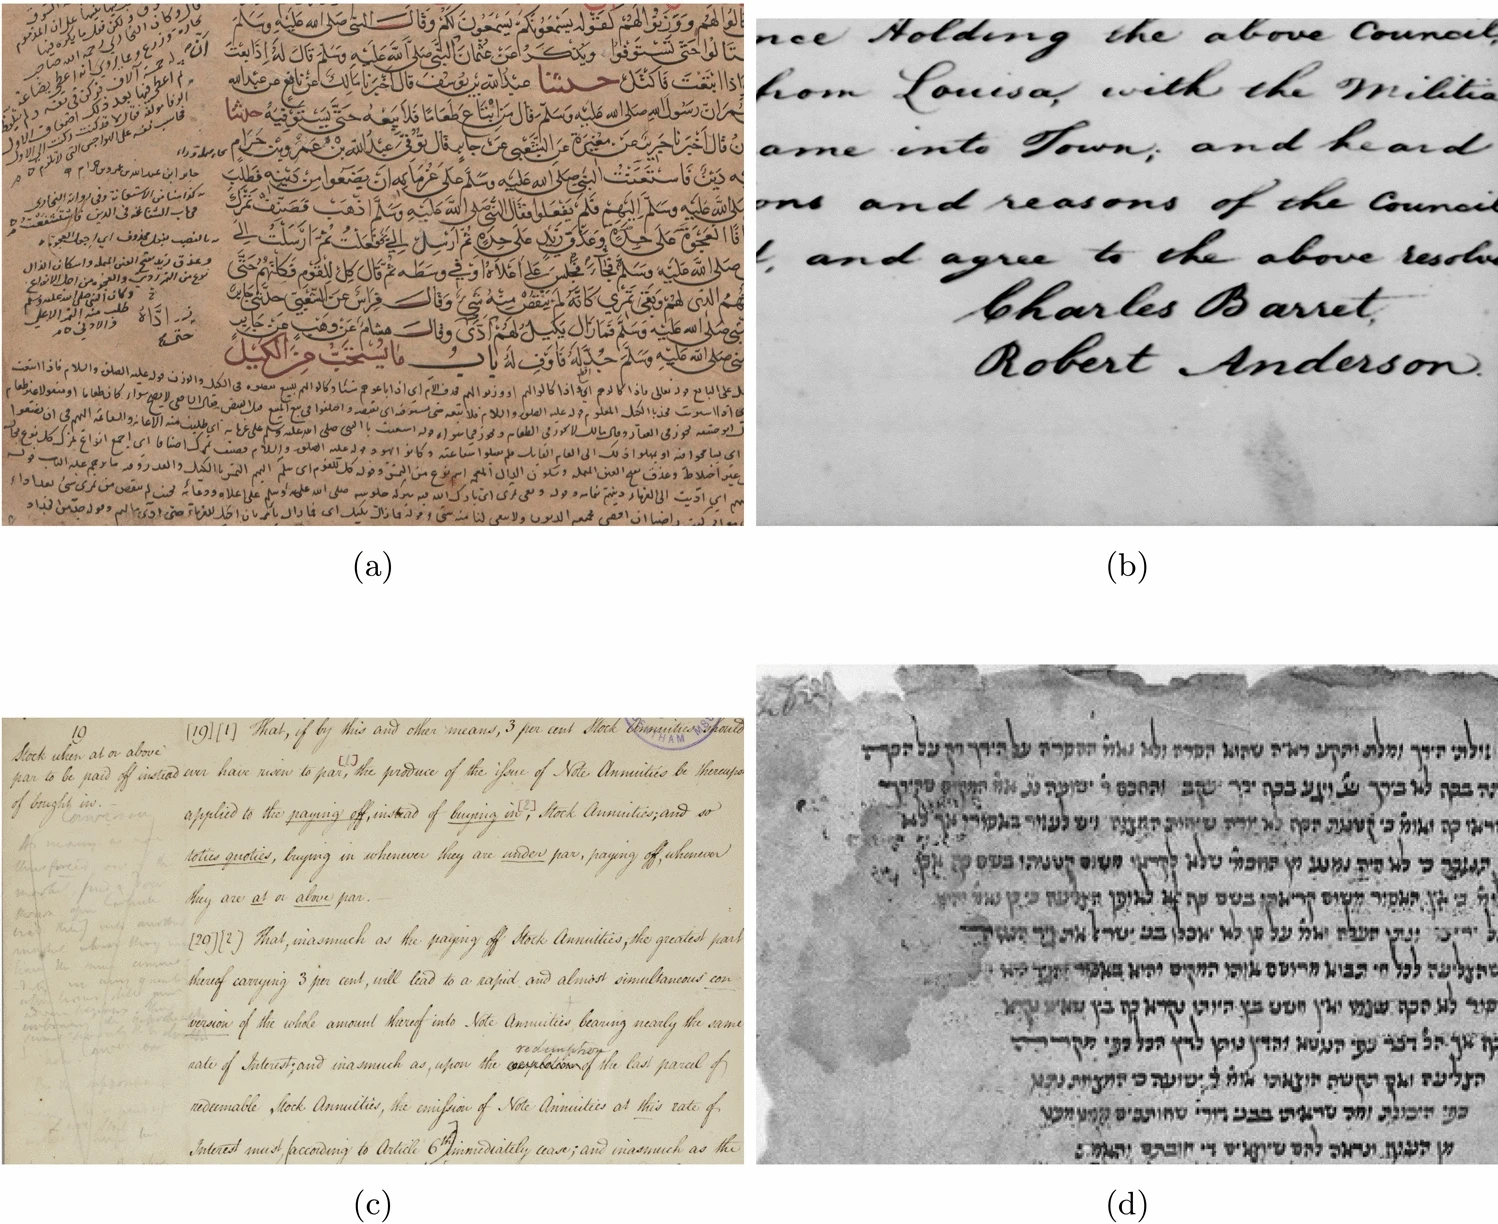
\includegraphics[width=\linewidth]{graphics/deg.png}
        \caption{Challenges in historical document layout analysis: irregular spaces, multi-oriented and fluctuating lines (a); marginal notes (a, c); stains (b, d); touching and connected characters (a, d); bleed-through (c), reproduced from \cite{Rabaev_Litvak_2025}.}
        \label{fig:hda_general_challenges}
    \end{subfigure}
    \hfill
    \begin{subfigure}[t]{0.48\linewidth}
        \centering
        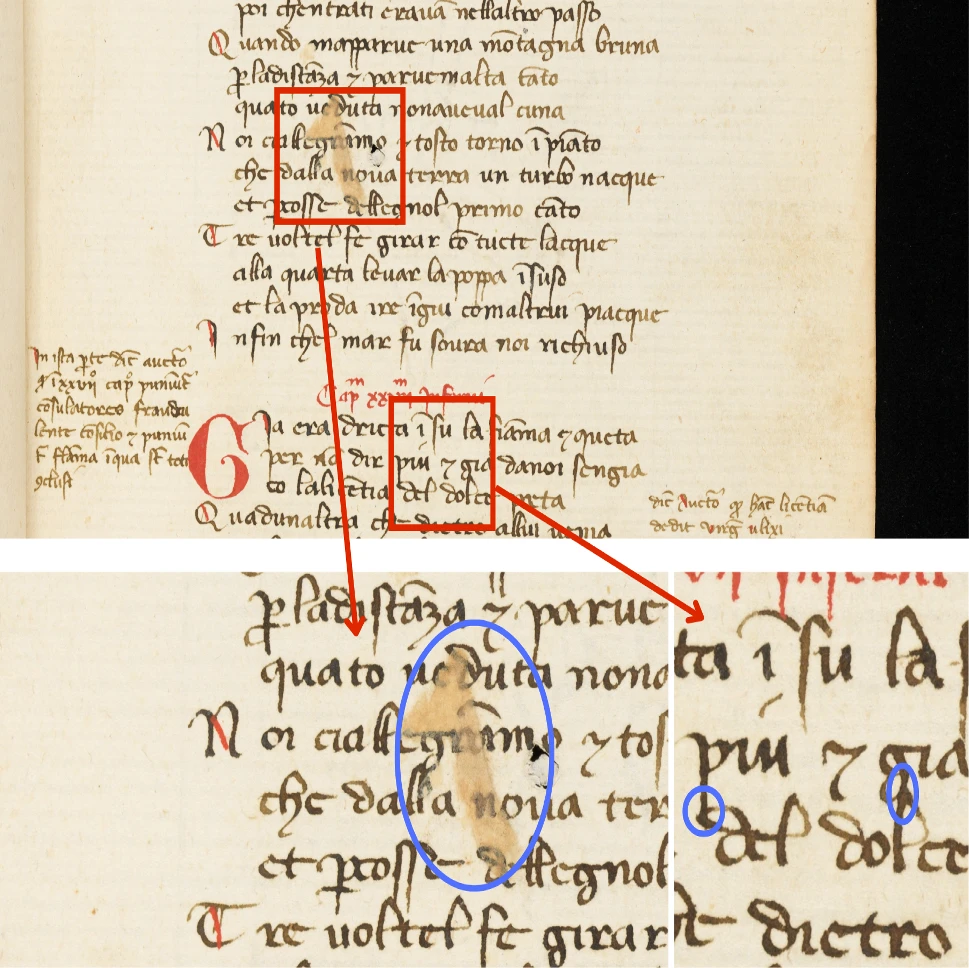
\includegraphics[width=\linewidth]{graphics/cb55_deg.png}
        \caption{Examples of overlapping and degraded text line regions from DIVA-HisDB \cite{diva_hisdb} CB55 subset, reproduced from \cite{Beghoura2026-dp}.}
        \label{fig:hda_line_challenges}
    \end{subfigure}

    \caption{Examples of challenges in text line segmentation in historical documents.}
    \label{fig:hda_challenges}
\end{figure}

Machine learning methods are used at every stage of the processing pipeline. In binarization, machine learning methods generally outperform traditional techniques, even under image degradation and acquisition issues such as uneven lighting; however, they have limitations, including reliance on large, diverse datasets, computational cost, and poor generalization to entirely new document degradations and styles \cite{jimaging11050133}. For document layout analysis, single-branch fully convolutional networks remain the main approach \cite{wu2025hooknet}. However, their reliance on pixel-wise labeled data remains a major limitation, since producing precise ground-truth annotations for historical manuscripts is time-consuming and costly \cite{De_Nardin_2023}. In \gls{htr}, current state-of-the-art approaches are largely transformer-based and tend to perform better on scripts whose handwriting style is similar to what the model was trained on. For instance, Titan and TrOCR-f often perform better out of the box on Latin-script materials, even though script-specific systems trained or fine-tuned on non-Latin data can ultimately achieve higher performance \cite{romein2025htr}. In this task, too, limited labeled domain data remains a key challenge \cite{Li2025}.

As shown in Figure \ref{fig:da_steps}, text line segmentation is the last step in the preprocessing phase; the quality of segmentation affects the performance of the downstream \gls{htr} task. Fizaine et al. measured this effect by comparing two segmentation models with postprocessing, using the same TrOCR \cite{DBLP:journals/corr/abs-2109-10282} detector fine-tuned on the DRoSb dataset, which they also used to train the segmentation models. As shown in Table \ref{tab:fizaine_ap_htr}, the Mask R-CNN \cite{he2017maskrcnn} model has better object-level metrics and also outperforms on the text recognition task, with a lower \gls{cer}.

\begin{table}[h]
    \centering
    \caption{Object-level text line segmentation performance, measured by \gls{ap}, and downstream \gls{htr} performance reported by Fizaine et al. \cite{fizaine}.}
    \label{tab:fizaine_ap_htr}
    \begin{tabular}{lcccc}
        \hline
        Model & \glsentryshort{ap}@0.5 & \glsentryshort{ap}@0.75 & \glsentryshort{ap}@[0.5,0.95] & \glsentryshort{cer} (\%) \\
        \hline
        Doc-UFCN \cite{boillet2021docufcn}
        & 0.62 & 0.52 & 0.50 & 15.3 \\
        Mask R-CNN \cite{he2017maskrcnn}
        & 0.96 & 0.85 & 0.78 & 4.2 \\
        \hline
    \end{tabular}
\end{table}

Text line segmentation is the main focus of this thesis and is discussed in Section~\ref{sec:tls}.

\section{Text Line Segmentation}
\label{sec:tls}

Text line segmentation aims to identify and separate individual text lines in a historical document image. Depending on the labeling method, a text line can be represented as a bounding box, a set of foreground pixels, a polygon surrounding the line, or a baseline. Figure \ref{fig:line_representation} illustrates how different representations describe the same handwritten text lines \cite{Textline_maskrcnn}.

\begin{figure}[H]
    \centering
    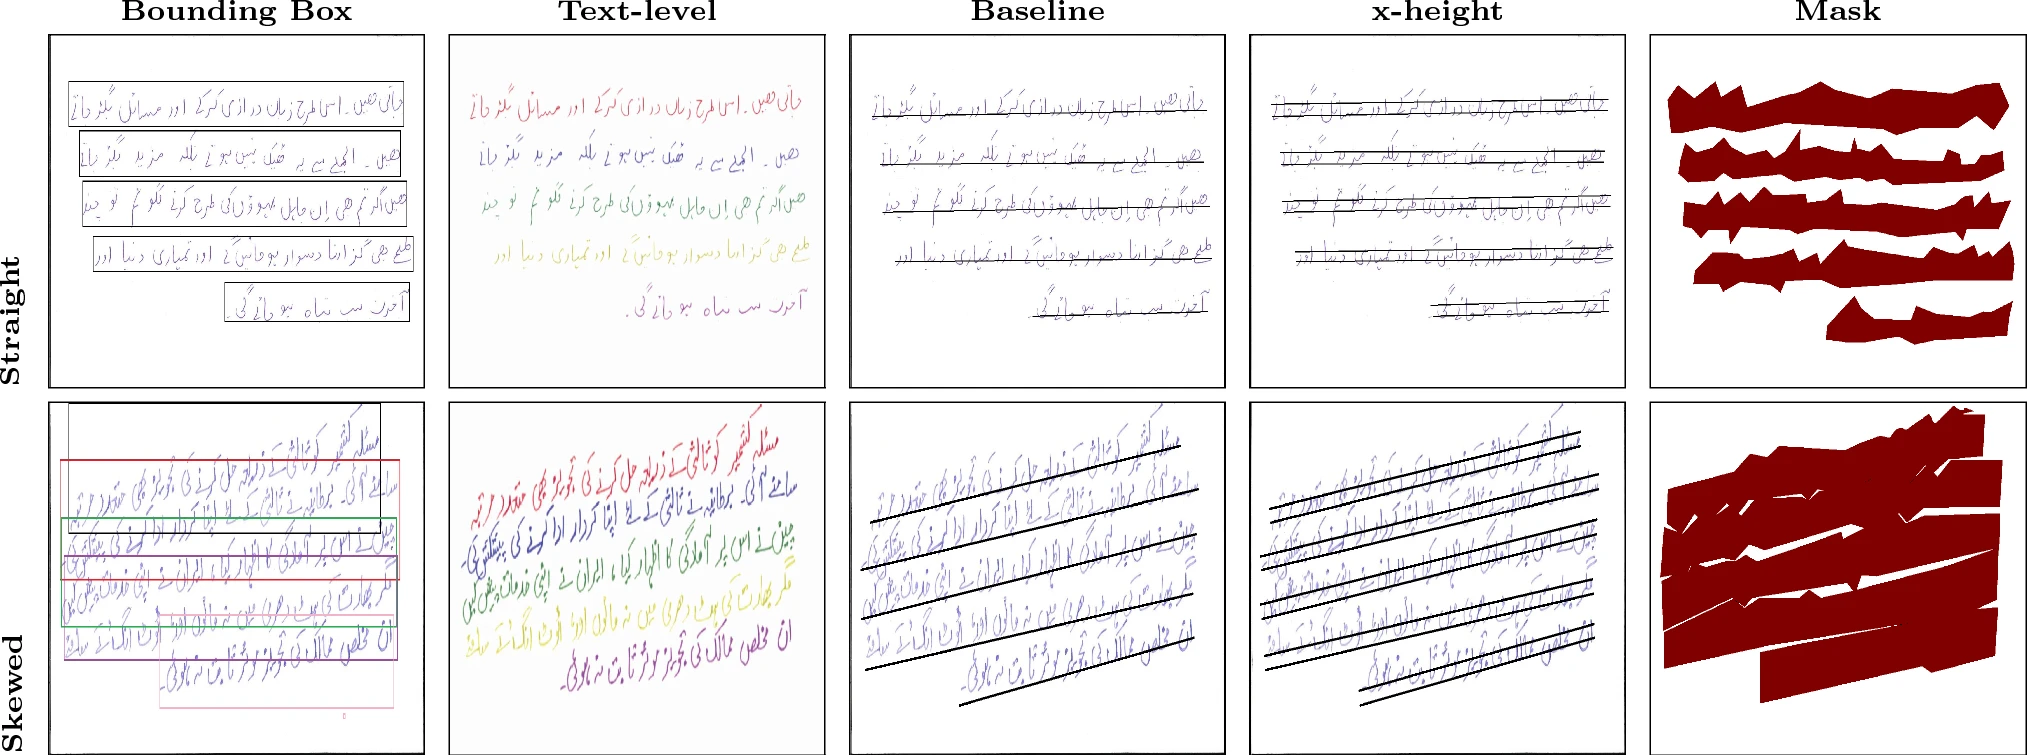
\includegraphics[width=0.85\linewidth]{graphics/tls_r.png}
    \caption{Different representations of a handwritten text line, reproduced from Islam et al. \cite{Textline_maskrcnn}.}
    \label{fig:line_representation}
\end{figure}

\paragraph{Unsupervised Methods} extract individual lines without manually annotated training data, which is very helpful when labeled data for historical documents is limited. The most recent works rely on handcrafted heuristics applied to document structure, such as including elongation analysis for line slicing \cite{sathik2021}, seam carving with specifically designed cost functions \cite{nguyen2022effective}, statistical gap analysis with unsupervised parameter estimation \cite{mukherjee2022unsupervised}, and clustering-based blob-line generation combined with energy minimization \cite{droby2022unsupervised}. Although supervised models are the minority of released models in recent years, as Rabaev et al. \cite{Rabaev_Litvak_2025} report, unsupervised methods achieve performance comparable to and even greater than state-of-the-art models, as can be seen from Table \ref{tab:unsupervised_diva_metrics}. However, their strong performance sometimes depends on the specific assumptions and characteristics of the document collections they are developed for, thus raising the question of whether such methods are robust. Hu et al. \cite{hu2021uchen} propose a method targeted specifically at Uchen Tibetan documents. In contrast, Nguyen et al. \cite{nguyen2022effective} and Droby et al. \cite{droby2022unsupervised} report strong, consistent results across different manuscript families. Additionally, these methods are usually computationally heavy, taking from 4 \cite{droby2022unsupervised} to approximately 30 minutes per page, depending on parameter configuration \cite{DBLP:journals/corr/abs-2003-08632}.

\begin{table}[H]
    \centering
    \caption{Comparison of unsupervised and supervised text line segmentation methods on the DIVA-HisDB \cite{diva_hisdb} dataset using \gls{pixeliu} and \gls{lineiu}.}
    \label{tab:unsupervised_diva_metrics}
    \begin{tabular}{llcc}
        \hline
        Model & Method & \glsentryshort{pixeliu} & \glsentryshort{lineiu} \\
        \hline
        Barakat et al. \cite{DBLP:journals/corr/abs-2003-08632}
        & Unsupervised & 97.50 & \textbf{99.46} \\

        Nguyen et al. \cite{nguyen2022effective}
        & Unsupervised & \textbf{99.36} & 98.86 \\

        Mask R-CNN \cite{Textline_maskrcnn}
        & Supervised & 96.00 & 98.40 \\
        \hline
    \end{tabular}
\end{table}

\paragraph{Supervised Methods} learn text line representations directly from annotated data, allowing them to capture visual characteristics that don't require creating any heuristics. In a recent survey \cite{Rabaev_Litvak_2025},
supervised and hybrid approaches dominate text line segmentation, with more instance segmentation methods published in recent years.

\begin{figure}[H]
    \centering
    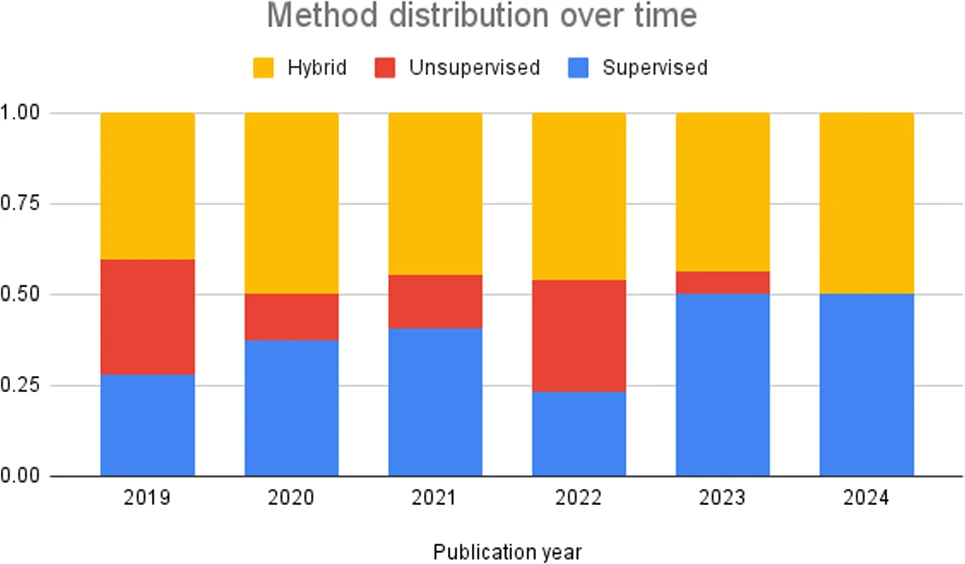
\includegraphics[width=0.85\linewidth]{graphics/sup_m.png}
    \caption{\Gls{tls} for historical manuscripts by approach over time, reproduced from Rabaev et al. \cite{Rabaev_Litvak_2025}.}
    \label{fig:methods}
\end{figure}

Supervised text line segmentation models fall into two categories: semantic segmentation, which may include postprocessing, and instance segmentation. Conventional \gls{fcn}-based models, such as Doc-UFCN \cite{boillet2021docufcn}, formulate the task as a two-class pixelwise classification with classes standing for background and text line. This approach works well when text lines are clearly separated, but neighboring or overlapping lines may be merged into the same foreground region and therefore require additional post-processing. More recent hybrid approaches, such as APAU-Net \cite{Beghoura2026-dp}, keep the semantic segmentation formulation but introduce explicit geometric prior heuristics describing the expected shape, position, and orientation of text lines. Instance segmentation methods address the separation problem differently. For example, Fizaine et al. \cite{fizaine} use Mask R-CNN and treat each text line as a separate object, predicting an individual mask for each detected line; this keeps neighboring lines as separate instances even when their regions are close or partially overlap, and it outperformed convolutional segmentation models, as can be seen from Table \ref{tab:fizaine_instance_comparison}.
\begin{table}[H]
    \centering
    \caption{Object-level text line segmentation performance reported by Fizaine et al. \cite{fizaine}.}
    \label{tab:fizaine_instance_comparison}
    \begin{tabular}{lccc}
        \hline
        Model & \glsentryshort{ap}@0.5 & \glsentryshort{ap}@0.75 & \glsentryshort{ap}@[0.5,0.95] \\
        \hline
        Doc-UFCN \cite{boillet2021docufcn}
        & 0.62 & 0.52 & 0.50 \\

        Mask R-CNN \cite{he2017maskrcnn}
        & \textbf{0.96} & \textbf{0.85} & \textbf{0.78} \\
        \hline
    \end{tabular}
\end{table}

\subparagraph{Robustness} across different scripts and document collections has been evaluated comparatively rarely. Islam et al. \cite{Textline_maskrcnn} study cross-script generalization by training their Mask R-CNN model only on the Urdu HUP dataset and evaluating it on eight other scripts. The model performs reasonably well on documents with layouts similar to the training data, but its performance drops by roughly 20--30\% on datasets with layouts the authors claim are non-similar. The largest failures occur on Arabic and German documents with very low inter-line spacing, showing that differences in page structure can still considerably affect cross-script generalization.

\subparagraph{Learning on a Small Amount of Data} has only recently become a research direction. Zottin et al. \cite{zottin2025exploring} first evaluated three established semantic segmentation architectures---\gls{fcn} \cite{long2015fully}, \gls{pspnet} \cite{zhao2017pyramid}, and DeepLabV3+ \cite{chen2018encoder}---on the U-DIADS-TL dataset, with only 3 annotated images. Their poor results showed rather potential for this field, as it was only baseline research in this paradigm.

The FEST competition \cite{Zottin_2025_FEST} has a wide range of solutions and showed that task-specific approaches can outperform the standard baselines. The winning PERO system used a ParseNet-based line detection pipeline followed by morphological post-processing. Another interesting submission, VAI-OCR, explicitly separated detection and segmentation into two stages: candidate text-line regions were first detected using a DBNet-style approach, after which individual cropped lines were segmented using an ensemble of U-Net and SegFormer models, which is particularly interesting, as to why such an intuitive approach is not used in text line segmentation. This thesis also developed a similar two-stage approach, described in Section \ref{sec:meth}.

U-Net-based architectures demonstrate strong results with very limited training data. Sterzinger et al. \cite{sterzinger2025fewshot} train a lightweight UNet++ model with a connection-aware loss with a \gls{lineiu} of 0.774 on U-DIADS-TL. More recently, APAU-Net \cite{Beghoura2026-dp} combines a residual U-Net with geometric priors and reaches an average \gls{lineiu} of 0.943 under the same three-page training setting.

However, these recent few-shot text line segmentation studies have been developed and evaluated only for the U-DIADS-TL dataset and have not been evaluated on other datasets. This leaves the behavior of few-shot \gls{tls} methods across different historical document collections comparatively underexplored.

\section{Few-shot Learning}
\label{sec:fsl}

\Gls{fsl} aims to learn from a small amount of labeled data \cite{fsl}, where the number of training instances, called shots  \(k\), typically \(k \in \{1,3,5,10\}\). In historical document analysis, this paradigm is highly relevant because of data limitations and the costs of labeling new ones. De Nardin et al. \cite{De_Nardin_2023}, proposed a few-shot framework in adjacent task of historical document layout analysis using only six annotated pages, two from each manuscript, instead of the complete 60-page training set of DIVA-HisDB \cite{diva_hisdb}. The data-poor method achieved performance comparable to data-rich approaches. Additionally, for scene text segmentation in natural images, Li et al. \cite{li2025tsalfewshottextsegmentation} proposed a model that creates prior knowledge from the pretrained \gls{clip} model \cite{DBLP:journals/corr/abs-2103-00020} to learn text attributes from only a few labeled images. On the TextSeg dataset \cite{xu2020rethinkingtextsegmentationnovel}, their 4-shot setting outperforms several many-shot baselines trained with up to 128 labeled examples, demonstrating the potential of few-shot methods for data-efficient text segmentation, even though the work is outside the historical document analysis domain. \Gls{fsl} can be applied in two approaches: meta-learning, where a model is trained to adapt rapidly to new tasks from a small support set, and transfer learning, where knowledge learned from a larger source dataset is reused for a target task with limited labeled data \cite{fsl}.

\paragraph{Transfer Learning using Pretrained Backbones}
 In deep neural networks, transfer learning is commonly implemented by initializing the model's feature extractor (i.e., the backbone/encoder) with pretrained weights and then adapting these weights to the target task through a brief training process called fine-tuning \cite{plested2026transfer}. This approach lets the feature extractor adjust representations learned from a larger source dataset rather than learning them entirely from limited target data.
 
Transfer Learning using Pretrained Backbones is available with both \glspl{cnn} and transformer-based models. ResNet-derived \glspl{cnn} have been adopted as generic feature extractors, whereas \Glspl{vit} have demonstrated state-of-the-art performance on large-scale computer vision benchmarks \cite{dosovitskiy2021imageworth16x16words}. Subsequent work on data-efficient training strategies further enhanced \gls{vit} performance under limited-data regimes \cite{touvron2021trainingdataefficientimagetransformers}. In parallel, ConvNeXt established that appropriately modernized convolutional architectures can achieve performance comparable to transformer-based approaches \cite{liu2022convnet2020s,woo2023convnextv2}. Later, self-supervised vision foundation models have provided general-purpose pretrained representations. DINOv2 uses \gls{vit} encoders pretrained on the LVD-142M dataset and provides features suitable for dense prediction tasks \cite{oquab2024dinov2learningrobustvisual,darcet2024visiontransformersneedregisters}. DINOv3 extends this family with both \gls{vit} and ConvNeXt encoders trained using the same self-supervised framework \cite{dinov3}.

Experiments with different backbones have also been performed in historical document analysis. Wödlinger and Sablatnig use an ImageNet-pretrained ResNet-50 as the encoder of a U-Net-based baseline detection system and report an F1 score of 0.881 on cBAD2019 \cite{wodlinger2021baseline}. Their experiments further show that improving the initial phase of model estimation improves final performance, with the F1 score increasing by ~10\% to 0.963 when ground-truth start points and angles are provided. Jindal and Ghosh \cite{jindal2023fasterrcnn} further replaced the conventional VGG-16 backbone of Faster R-CNN with ResNet-50 for ancient handwritten text line segmentation and report an F-measure of 99.98\%, outperforming the original Faster R-CNN configuration. Fizaine et al. \cite{fizaine} also suggest replacing the backbone in their Mask R-CNN implementation with a more recent architecture, such as ConvNeXt \cite{woo2023convnextv2}, to potentially improve both accuracy and processing speed. These works suggest room for extensive research on \gls{tls} backbones.
The source of pretraining also matters. Common backbones are pretrained on large
datasets such as ImageNet \cite{deng2009imagenet} and \gls{coco} \cite{DBLP:journals/corr/LinMBHPRDZ14}, whereas historical document datasets such as \gls{cbad} \cite{cbad-2019} and CATMuS \cite{catmus-medieval} are substantially smaller but closer to the target domain. Table \ref{tab:pretraining_datasets} demonstrates an order-of-magnitude difference between the generic and task-specific datasets.

\begin{table}[H]
    \centering
    \caption{Size comparison of generic computer vision and historical document datasets relevant for pretraining.}
    \label{tab:pretraining_datasets}
    \begin{tabular}{llr}
        \hline
        Dataset & Domain & Number of images/pages \\
        \hline
        ImageNet \cite{deng2009imagenet}
        & Natural images & 14,197,122 images \\

        ImageNet-1K
        & Natural images & 1,281,167 images \\

        \gls{coco} \cite{DBLP:journals/corr/LinMBHPRDZ14}
        & Natural images & 328,000 images \\

        \gls{cbad} 2019 \cite{cbad-2019}
        & Historical documents & 3,021 pages \\

        CATMuS Medieval \cite{catmus-medieval}
        & Historical documents & 1,705 images \\
        \hline
    \end{tabular}
\end{table}

Domain-specific encoder pretraining remains unexplored for \gls{tls}. De Nardin et al. \cite{denardin2025indomain} show that pretraining source strongly affects historical document layout analysis. On CB55, training from scratch yields 43.9\% \gls{iou} and 57.6\% F1; hybrid \gls{coco}+U-DIADS-Bib pretraining raises this to 50.8\% \gls{iou} and 65.1\% F1 with a frozen encoder, and 54.6\% \gls{iou} and 69.0\% F1 after fine-tuning—gains of up to +10.7 \gls{iou} and +11.4 F1 points, proving the potential of this approach for \gls{tls}.

\section{Summary of Studies and Research Gap}

Recent work therefore suggests that both encoder architecture and pretraining strategy can affect performance under limited data. However, a systematic comparison of modern convolutional, Transformer-based, and vision-foundation-model encoders under the same few-shot text line segmentation setting, alongside different encoder pretraining options, remains unexplored, although these methods are used for adjacent tasks in historical layout analysis. This motivates the controlled comparison in this thesis, with the \glspl{rq} stated in Section \ref{ch:rqs}.
